\documentclass[11pt]{article}
\usepackage[T1]{fontenc}
\usepackage{lmodern}
\usepackage[margin=1.08in]{geometry}
\usepackage{amsmath,amssymb,amsthm,mathtools}
\usepackage{graphicx}
\usepackage{microtype}
\usepackage{xcolor}
\usepackage{hyperref}
\hypersetup{colorlinks=true,linkcolor=blue!45!black,citecolor=green!35!black,urlcolor=blue!55!black,pdftitle={Sharp one-dimensional Lieb--Thirring inequalities for matrix potentials},pdfauthor={OpenAI}}
\newtheorem{theorem}{Theorem}[section]
\newtheorem{proposition}[theorem]{Proposition}
\newtheorem{lemma}[theorem]{Lemma}
\newtheorem{corollary}[theorem]{Corollary}
\theoremstyle{definition}
\newtheorem{definition}[theorem]{Definition}
\theoremstyle{remark}
\newtheorem{remark}[theorem]{Remark}
\newcommand{\R}{\mathbb R}
\newcommand{\C}{\mathbb C}
\newcommand{\HS}{\mathrm{HS}}
\DeclareMathOperator{\tr}{tr}
\DeclareMathOperator{\Tr}{Tr}
\DeclareMathOperator{\Sym}{Sym}
\DeclareMathOperator{\sech}{sech}
\DeclareMathOperator{\diag}{diag}
\DeclareMathOperator{\op}{op}
\numberwithin{equation}{section}
\allowdisplaybreaks[2]
\setlength{\emergencystretch}{1.5em}

\title{Sharp one-dimensional Lieb--Thirring inequalities\newline for matrix potentials}
\author{OpenAI}
\date{October 5, 2026}
\begin{document}
\maketitle
\begin{abstract}
We prove the sharp one-dimensional Lieb--Thirring inequality for every finite
matrix size and every exponent $1/2<\gamma<3/2$. The optimal constant is the
scalar one-bound-state constant, independently of the matrix size. The
inequality bounds the full sum of negative eigenvalue moments for every
measurable Hermitian positive semidefinite potential $W$ satisfying
$\int_\R\tr(W^{\gamma+1/2})<\infty$. The matrices may have arbitrary rank and
need not commute at different points.
\end{abstract}
\tableofcontents
\section{Introduction}\label{sec:introduction}

Lieb--Thirring inequalities bound moments of the negative eigenvalues of a Schr\"odinger operator by an integral of its potential. Their sharp constants measure how much binding is possible for a prescribed potential cost. When the wave function has several components, the potential becomes a matrix, and its eigenspaces may change with position. The question addressed here is whether this additional freedom increases the optimal constant in one dimension.

Let $m\ge1$, let $1/2<\gamma<3/2$, and put $p=\gamma+1/2$.
For a measurable Hermitian positive semidefinite matrix function
$W:\R\to\C^{m\times m}$ satisfying
\begin{equation}\label{eq:potential-class}
  \int_\R\tr(W(x)^p)\,dx<\infty,
\end{equation}
consider the quadratic form
\begin{equation}\label{eq:schrodinger-form}
 h_W[\psi]=\int_\R\|\psi'(x)\|^2\,dx
       -\int_\R\langle\psi(x),W(x)\psi(x)\rangle\,dx,
 \qquad \psi\in H^1(\R;\C^m).
\end{equation}
This form is closed and bounded below. Its self-adjoint operator is denoted by
$H_W=-d^2/dx^2-W$. Its negative spectrum consists of eigenvalues, with finite
multiplicities and possible accumulation only at zero; these facts are proved
under exactly \eqref{eq:potential-class} in Section~\ref{sec:spectral}.
We write
\[
 \Tr(H_W)_-^\gamma=\sum_{\lambda_j(H_W)<0}|\lambda_j(H_W)|^\gamma,
\]
initially allowing the sum to be infinite. Matrix powers are defined by spectral
functional calculus, and $\tr$ is the ordinary, unnormalized matrix trace.

\begin{theorem}[Sharp matrix inequality]\label{thm:main}
For every $1/2<\gamma<3/2$, every finite $m\ge1$, and every $W$ satisfying
\eqref{eq:potential-class},
\begin{equation}\label{eq:main-bound}
 \Tr(H_W)_-^\gamma\le C_\gamma\int_\R\tr(W(x)^{\gamma+1/2})\,dx,
 \qquad
 C_\gamma=
 \left(\frac{\gamma-1/2}{\gamma+1/2}\right)^{\gamma-1/2}
 \frac{\Gamma(\gamma+1)}{\sqrt\pi\,\Gamma(\gamma+3/2)}.
\end{equation}
The constant is optimal in every matrix dimension. With
$r=(\gamma-1/2)^{-1}$, it is attained by
\begin{equation}\label{eq:extremal-potential}
 W(x)=\diag\big((r+1)\sech^2(rx),0,\ldots,0\big).
\end{equation}
\end{theorem}

The matrices $W(x)$ may be noncommuting and may have arbitrary rank. In
particular, the conclusion concerns changing internal channels as well as
independent scalar channels.

\subsection{Historical context and relationship to prior work}
Lieb and Thirring introduced their eigenvalue inequalities in the study
of fermionic kinetic energy and the stability of matter
\cite{LiebThirring1975,LiebThirring1976}.
The one-state variational problem goes back to Keller \cite{Keller1961}.
In one dimension its optimal constant exceeds the semiclassical constant
for $1/2<\gamma<3/2$. The scalar conjecture in this interval asks whether
summing all negative eigenvalues changes that one-state constant.
The companion paper \cite[Theorem~1.1]{ScalarCompanion} proves that it does
not. The present paper establishes the same constant for arbitrary finite
matrix size, allowing the eigenspaces of the potential to vary with position.

Sharp matrix inequalities at the two endpoint exponents have an
established history. Weidl proved finiteness at the scalar lower endpoint
\cite{Weidl1996}, and Hundertmark, Lieb and Thomas obtained the sharp
$\gamma=1/2$ inequality with constant $1/2$
\cite[Theorem~1]{HLT1998}; Hundertmark, Laptev and Weidl proved the
operator-valued version \cite[Theorem~3.1]{HLW2000}.
At $\gamma=3/2$, Laptev and Weidl established the sharp matrix estimate by
trace identities and extended it to operator-valued potentials
\cite[Theorems~2.1 and~2.2]{LaptevWeidl2000}.
Aizenman--Lieb integration in the spectral parameter gives the larger
exponents \cite{AizenmanLieb1978}. Laptev and Weidl's dimension-lifting
argument then yields the semiclassical constant in every spatial dimension
for $\gamma\ge3/2$ \cite[Theorem~3.1]{LaptevWeidl2000}.
Benguria and Loss gave a proof of the matrix upper-endpoint estimate by
Riccati factorization and commutation \cite{BenguriaLoss2000}.

In the open interval, Hundertmark, Laptev and Weidl obtained the
operator-valued upper bound with twice the semiclassical constant
\cite[Theorem~4.1]{HLW2000}.
Dolbeault, Laptev and Loss developed the method of orthonormal
vector-valued functions at exponent one
\cite[Theorems~1 and~3]{DLL2008}.
More recently, Read and Schulz proved the sharp value
$4/(3\sqrt3\pi)$ for $\gamma=1$, including operator-valued potentials
\cite[Proposition~4 and Equation~(2.1)]{ReadSchulz2026}.
Thus the exponent-one case of our theorem is already contained in their
result. Our additional range is $1/2<\gamma<3/2$, $\gamma\ne1$.

The proof adapts the finite-interval action and continuation framework
of \cite[Theorem~2.1, Proposition~5.1 and Section~6]{ScalarCompanion}.
The companion's comparison applies when the pointwise density has rank
at most one \cite[Proposition~4.1]{ScalarCompanion}.
The new analytic step removes that restriction, making the action method
applicable to vector-valued wave functions.



\subsection{The matrix comparison and the proof strategy}
The proof uses the finite-interval action method of the scalar companion
\cite{ScalarCompanion}. To explain the extension, choose finitely many
orthonormal real vector-valued trial functions $u_1,\ldots,u_n$ and place them in
the rows of a matrix function $U(x)$. A lower triangular coefficient matrix
$C$ produces $A(x)=CU(x)$, so that the $i$th row of $A$ remains in the span
of $u_1,\ldots,u_i$. For trial functions ordered by their negative energies,
this preserves the spectral inequalities needed to bound the action from above.
The action subtracts a power of the matrix density
$\rho(x)=A(x)A(x)^{\mathsf T}$, and a complementary lower bound recovers
the sum of the chosen eigenvalue moments. A fixed realification of the
potential will subsequently give the complex Hermitian case.

The lower bound is obtained by connecting two prescribed diagonal matrices
$K$ and $-K$, where the diagonal entries of $K$ are the positive square roots
of the absolute values of the negative trial energies. A regularized matrix field $M$ drives an equation with the
penalized constraint $M(B)=\rho$. In the scalar-potential argument,
$A$ has one column and this constraint has rank at most one. For matrix
potentials, $\rho$ can have any rank. The essential new estimate controls
$\tr(\rho^q)$ in this setting, where $q$ is conjugate to $p$.

We prove that estimate as an independent result in Section~\ref{sec:trace}.
For Hermitian $B,V$ such that $(sI-B)^2+V$ is uniformly positive for real $s$,
we form a weighted integral $N$ of resolvent differences. When $N\ge0$,
the result is $\tr(NV)\ge\tr(N^q)$. The hypothesis permits indefinite $V$,
which is necessary when $V$ is later obtained from $K^2-B^2$.
Half-line solutions of a constant-coefficient differential equation give
two boundary matrices. Their sum identifies the integrated resolvent,
and their difference accounts for the noncommutative error. A logarithmic
determinant identity and a nonnegative matrix square then prove the trace
comparison with the required constant.

Section~\ref{sec:action-framework} states the action inequality and isolates
its relation to spectral estimates. Sections~\ref{sec:field}--\ref{sec:action-limit}
construct the field, connect the endpoints, and remove the penalty. The
continuation argument works modulo independent signs of the rows of $C$.
After smoothing and perturbation, parity of the boundary of the quotient
zero set forces an endpoint solution. Finally,
Section~\ref{sec:spectral} applies the action inequality to smooth trial
spaces and passes to general potentials and the full spectral moment.
All of these steps are proved here; the companion is cited for the method
and its scalar specialization.

\subsection{Conventions}
For the rest of the paper we use
\begin{equation}\label{eq:exponents}
 \sigma=\gamma-\tfrac12\in(0,1),\qquad
 p=1+\sigma,\qquad q=1+\sigma^{-1},\qquad
 \beta=\sigma-\tfrac12.
\end{equation}
Thus $p^{-1}+q^{-1}=1$. The identity matrix has the size specified by its
context. On matrices we use the Hilbert--Schmidt norm
$\|A\|_{\HS}^2=\tr(A^*A)$ and the operator norm $\|A\|_{\op}$.
The space $\Sym_n$ of real symmetric matrices carries the inner product
$\tr(BH)$. Complex inner products are linear in the second variable.

\section{The finite-interval action inequality}\label{sec:action-framework}

We first formulate the lower bound on the variational action that will
lead to an upper bound on spectral moments. Let $\Omega=(x_-,x_+)$ be a bounded interval,
let $n,d\ge1$, and suppose
\begin{equation}\label{eq:row-orthonormality}
 U\in H^1_0(\Omega;\R^{n\times d}),\qquad
 \int_\Omega U(x)U(x)^{\mathsf T}\,dx=I_n.
\end{equation}
Thus the rows of $U$ are orthonormal as $\R^d$-valued functions. Fix
$K=\diag(k_1,\ldots,k_n)$ with each $k_i>0$. For
$A\in H^1_0(\Omega;\R^{n\times d})$ define
\begin{equation}\label{eq:action}
 \mathcal E(A)=\int_\Omega
 \left(\|A'\|_{\HS}^2+\tr(K^2AA^{\mathsf T})
                  -\tr((AA^{\mathsf T})^q)\right)\,dx.
\end{equation}
This integral is finite, since one-dimensional $H^1$ functions on a bounded
interval are continuous. Write $\mathcal L$ for the real lower triangular
$n\times n$ matrices.

\begin{theorem}[Action inequality]\label{thm:action}
For every $0<\sigma<1$ and all the data just specified,
\begin{equation}\label{eq:action-bound}
 \sup_{C\in\mathcal L}\mathcal E(CU)
 \ge\sum_{i=1}^n\int_{-k_i}^{k_i}(k_i^2-s^2)^\sigma\,ds.
\end{equation}
\end{theorem}

The order of the $k_i$ is immaterial for this theorem. For its spectral
application we order them decreasingly: lower triangularity then preserves
the nested trial spaces on which the form is at most $-k_i^2$ times the
squared norm. Matrix Young duality bounds the action from above by a constant
times $\int\tr(W^p)$, while
\[
 \int_{-k_i}^{k_i}(k_i^2-s^2)^\sigma\,ds
 =\mathrm B(\tfrac12,1+\sigma)k_i^{2\sigma+1}
\]
has exactly the desired spectral exponent. Section~\ref{sec:spectral}
gives this deduction, including its approximation steps.

The scalar companion proves the version with $d=1$
\cite[Theorem~2.1]{ScalarCompanion}. Its field and endpoint construction
also suggest the present proof. The necessary new ingredient is an
inequality for positive matrix densities of unrestricted rank. We prove
that comparison next, before constructing the regularized field to which
it applies. The proof of Theorem~\ref{thm:action} is completed in
Section~\ref{sec:action-limit}.

\section{An integrated matrix trace inequality}\label{sec:trace}

The matrix step in the proof compares an integrated resolvent
difference with the Hermitian perturbation that produces it.
We prove the comparison for matrices of arbitrary size.  The
perturbation may be indefinite; positivity is imposed on the entire
symbol.

For the fixed exponent $0<\sigma<1$, define $c_\sigma>0$ by
\begin{equation}\label{eq:trace-normalization}
 c_\sigma^{-1}
 =\int_0^\infty t^\beta
       \bigl(t^{-1/2}-(t+1)^{-1/2}\bigr)\,dt.
\end{equation}
Recall that $\beta=\sigma-\tfrac12\in(-\tfrac12,\tfrac12)$.
The integrand in \eqref{eq:trace-normalization} is
$O(t^{\beta-1/2})$ at zero and $O(t^{\beta-3/2})$ at infinity.
The integral is therefore finite, and scaling gives
\begin{equation}\label{eq:trace-scaling}
 c_\sigma\int_0^\infty t^\beta
       \bigl(t^{-1/2}-(t+y)^{-1/2}\bigr)\,dt=y^\sigma,
 \qquad y\geq0.
\end{equation}

\begin{theorem}[Integrated trace comparison]\label{thm:trace}
Let $n\geq1$ and let $B,V\in\C^{n\times n}$ be Hermitian.
Suppose that for some $b>0$,
\begin{equation}\label{eq:trace-symbol}
 Y_s=(sI-B)^2,\qquad X_s=Y_s+V\geq bI
 \qquad\text{for every }s\in\R.
\end{equation}
For $t>0$, set
\begin{equation}\label{eq:trace-resolvents}
 R(t)=\frac1\pi\int_\R(X_s+tI)^{-1}\,ds,
 \qquad P(t)=t^{-1/2}I-R(t),
\end{equation}
and define
\begin{equation}\label{eq:trace-N}
 N=c_\sigma\int_0^\infty t^\beta P(t)\,dt.
\end{equation}
These integrals converge absolutely in matrix norm.  If $N\geq0$, then
\begin{equation}\label{eq:trace-comparison}
                         \tr(NV)\geq\tr(N^q).
\end{equation}
\end{theorem}

For a scalar $V=v>0$, shifting the variable $s$ gives
$R(t)=(t+v)^{-1/2}$ and $N=v^\sigma$.  Thus the two sides of
\eqref{eq:trace-comparison} agree in the scalar case.  To retain this
constant for noncommuting matrices, we will express the difference in
\eqref{eq:trace-comparison} as an integral of nonnegative terms.
The first step computes the resolvent through solutions of a
constant-coefficient equation on the two half-lines.

\subsection{Resolvent estimates and half-line solutions}

We first verify convergence.  The matrices $X_s$ and $Y_s$ grow
quadratically as $|s|\to\infty$.  Combined with the lower bound in
\eqref{eq:trace-symbol}, this shows that $X_s^{-1}$ has an integrable
matrix-norm bound on $\R$.  Consequently $R(t)>0$ and $R(t)=O(1)$ as
$t\downarrow0$.  Diagonalizing $B$ gives
\[
 \frac1\pi\int_\R(Y_s+tI)^{-1}\,ds=t^{-1/2}I.
\]
For $t\geq1$, both $X_s+tI$ and $Y_s+tI$ are bounded below by
$c(s^2+t)I$ for some $c>0$ independent of $s,t$.  The resolvent
identity, with the fixed matrix difference $V$, therefore gives
\begin{equation}\label{eq:trace-P-bounds}
 \|P(t)\|=
 \begin{cases}
  O(t^{-1/2}),&t\downarrow0,\\
  O(t^{-3/2}),&t\to\infty.
 \end{cases}
\end{equation}
For the second estimate, the norm of the difference of the two
resolvents is at most $C(s^2+t)^{-2}$, whose $s$-integral is
$O(t^{-3/2})$.  The range of $\beta$ now proves the absolute
convergence in \eqref{eq:trace-N}.

Matrix Riccati equations also underlie the commutation approach to
matrix Schr\"odinger inequalities \cite{BenguriaLoss2000}.  Here the
boundary matrices will compute both a resolvent integral and a
logarithmic determinant integral.  Fix $t>0$, write
$\nabla=\partial_x-iB$, and consider
\begin{equation}\label{eq:trace-ode}
                    (-\nabla^2+V+tI)\psi=0.
\end{equation}
The following construction relates its decaying solutions to $R(t)$.

\begin{lemma}\label{lem:trace-half-lines}
For every $v\in\C^n$, equation \eqref{eq:trace-ode} has a unique
$H^1$ solution on each half-line with boundary value $v$ at zero.
There are Hermitian matrices $S=S(t)$ and $T=T(t)$ such that these
solutions satisfy
\begin{equation}\label{eq:trace-boundary-maps}
 \nabla\psi(0+)=-Sv,\qquad \nabla\psi(0-)=Tv,
\end{equation}
respectively.  They obey
\begin{equation}\label{eq:trace-riccati}
 V+tI=S^2+i[B,S]=T^2-i[B,T],
 \qquad \frac{S+T}{2}=R(t)^{-1}.
\end{equation}
Every eigenvalue of $B+iS$ has strictly positive imaginary part.
\end{lemma}

\begin{proof}
With inner products linear in the second argument, let
\[
 a_t(\phi,\psi)=\int
    \bigl(\langle\nabla\phi,\nabla\psi\rangle
       +\langle\phi,(V+tI)\psi\rangle\bigr)\,dx.
\]
On the full line its Fourier symbol is $X_s+tI$, and
\eqref{eq:trace-symbol} and quadratic growth give
$X_s+tI\geq c_t(1+s^2)I$ for some $c_t>0$.
Thus $a_t$ is coercive on $H^1(\R;\C^n)$.  Zero extension proves
the same assertion on the subspace of $H^1$ functions on either
half-line whose boundary trace is zero.

Choose any $H^1$ extension $\eta$ of the prescribed boundary value.
On the trace-zero space the form $a_t$ is an equivalent Hilbert
space inner product.  The Riesz representation theorem gives a
unique correction $u$ in that space with
$a_t(\phi,u)=-a_t(\phi,\eta)$ for every trace-zero $\phi$.
Then $\psi=\eta+u$ solves \eqref{eq:trace-ode} weakly.
Conversely, an $H^1$ solution satisfies this weak identity by
density of interior test functions in the trace-zero space, so
coercivity proves uniqueness.

The equation implies $\psi''\in L^2$.  In particular the solutions
belong to $H^2$, their first derivatives have boundary traces, and
both $\psi$ and $\psi'$ tend to zero at the infinite end of the
half-line.  Define $S$ and $T$ by \eqref{eq:trace-boundary-maps}.
For the right solutions with data $v,w$, integration by parts gives
$a_t(\psi_v,\psi_w)=\langle v,Sw\rangle$; on the left it gives
$a_t(\psi_v,\psi_w)=\langle v,Tw\rangle$.  Since $a_t$ is Hermitian,
both boundary matrices are Hermitian.

Translation and uniqueness imply the same derivative relations
at every interior point:
\[
 \nabla\psi=-S\psi\quad\text{on }(0,\infty),\qquad
 \nabla\psi=T\psi\quad\text{on }(-\infty,0).
\]
For example,
$\nabla(-S\psi)=-S\nabla\psi+i[B,S]\psi$.
Substitution into \eqref{eq:trace-ode}, followed by evaluation at
zero for arbitrary boundary data, proves the two Riccati identities
in \eqref{eq:trace-riccati}.

Glue the right and left solutions with the same value $v$ at zero.
Figure~\ref{fig:half-line-gluing} records the boundary signs and
the normalization in this gluing identity.
The resulting function is continuous, and its derivative has jump
$-(S+T)v$.  On the full line it therefore satisfies
\[
 (-\nabla^2+V+tI)\psi=\delta_0(S+T)v.
\]
Using the Fourier transform with forward kernel $e^{-isx}$ and
inverting at zero gives
\[
 v=\frac1{2\pi}\int_\R(X_s+tI)^{-1}\,ds\,(S+T)v
   =\frac12R(t)(S+T)v.
\]
This inversion may first be taken in tempered distributions;
the transformed function is integrable because the inverse symbol
is $O(s^{-2})$, so evaluation at zero is legitimate.  Since
$R(t)>0$, the second identity in \eqref{eq:trace-riccati} follows.

Finally the right solutions satisfy $\psi'=i(B+iS)\psi$.
If $(B+iS)v=zv$ with $v\ne0$, uniqueness for this first-order
initial-value problem gives $\psi(x)=e^{izx}v$.
It belongs to $L^2(0,\infty;\C^n)$, hence
$\operatorname{Im}z>0$.
\end{proof}

\begin{figure}[tb]
 \centering
 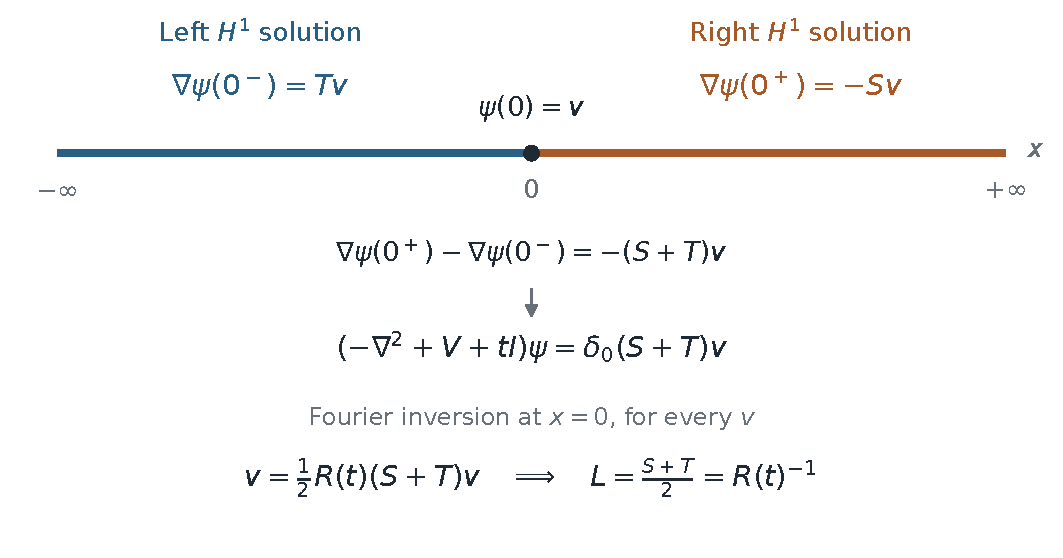
\includegraphics[width=\linewidth]{figures/half-line-gluing.pdf}
 \caption{Gluing the two half-line solutions at a common boundary
 value $v$, for fixed $t>0$ and $\nabla=\partial_x-iB$.
 The colored segments represent the two domains, rather than scalar
 solution profiles.  The jump of the covariant derivative gives the
 point source $\delta_0(S+T)v$.  Fourier inversion at zero, for every
 $v$, identifies the averaged boundary map $(S+T)/2$ with $R(t)^{-1}$.
 The separate Hermitian matrices $S$ and $T$ need not be positive.}
 \label{fig:half-line-gluing}
\end{figure}

Define the Hermitian matrices
\begin{equation}\label{eq:trace-LZ-definition}
 L=\frac{S+T}{2}=R(t)^{-1}>0,
 \qquad Z=\frac{S-T}{2}.
\end{equation}
Adding and subtracting the Riccati identities gives
\begin{equation}\label{eq:trace-LZ-identities}
 V+tI=L^2+Z^2+i[B,Z],\qquad
 LZ+ZL+i[B,L]=0.
\end{equation}
In an eigenbasis of $L$, the second identity has diagonal entries
$2L_{jj}Z_{jj}=0$.  Thus $\tr Z=0$.
Multiplying that identity on both sides by $R=L^{-1}$ gives
$i[R,B]=-(ZR+RZ)$, and cyclicity of the trace yields
\[
 i\tr(R[B,Z])=i\tr([R,B]Z)=-2\tr(RZ^2).
\]
Consequently
\begin{equation}\label{eq:trace-RV}
                 \tr\bigl(R(V+tI)\bigr)=\tr L-\tr(RZ^2).
\end{equation}
The correction $\tr(RZ^2)=\tr(ZRZ)$ is nonnegative.

We have expressed the integrated resolvent through $L$ and identified
a nonnegative correction involving $Z$.  To compare the weighted
integral $N$ with $V$, we next need a scalar quantity whose
$t$-derivative contains $\tr R(t)$.  The logarithm of the determinant
provides that quantity, and the same half-line matrices evaluate it.

\subsection{The logarithmic integral and its weighted identity}

Define
\begin{equation}\label{eq:trace-F-definition}
 F(t)=\frac{\tr V}{\sqrt t}
       -\frac1\pi\int_\R
          \log\frac{\det(X_s+tI)}{\det(Y_s+tI)}\,ds.
\end{equation}
The determinants are positive.  Factoring with
$(Y_s+tI)^{1/2}$ shows that the log ratio is $O(|s|^{-2})$ at
infinity, so its integral converges absolutely.  Its $t$-derivative
is the trace of the difference of the two resolvents.  This has an
integrable bound locally uniform for $t>0$, by the same resolvent
identity used above.  In particular $F$ is continuously
differentiable on $(0,\infty)$.

The first Riccati identity gives the factorization
\begin{equation}\label{eq:trace-factorization}
             X_s+tI=(sI-B+iS)(sI-B-iS).
\end{equation}
Let $u_j+iv_j$, $1\leq j\leq n$, be the eigenvalues of $B+iS$,
with algebraic multiplicity.  Lemma~\ref{lem:trace-half-lines}
gives $v_j>0$.  Since $B-iS=(B+iS)^*$, taking determinants in
\eqref{eq:trace-factorization} gives
\[
 \det(X_s+tI)=\prod_{j=1}^n\bigl((s-u_j)^2+v_j^2\bigr).
\]
The denominator in \eqref{eq:trace-F-definition} has the same form,
with centers the eigenvalues of $B$ and widths all equal to
$\sqrt t$.

These centers can be removed when integrating with symmetric
cutoffs.  Indeed, for $h(s)=\log(s^2+v^2)$, the function $h$ is
even and $h'(s)\to0$ at both ends.  For a fixed translation $a$,
\[
 \frac{d}{da}\int_{-r}^r h(s-a)\,ds=h(r+a)-h(r-a)\longrightarrow0
 \quad(r\to\infty),
\]
uniformly for $a$ in bounded intervals.  Integrating in $a$ shows
that the translation changes the symmetric-cutoff integral by a
quantity tending to zero.  After centering the factors, the scalar
identity
\[
 \int_\R\log\frac{s^2+v^2}{s^2+w^2}\,ds=2\pi(v-w),
 \qquad v,w>0,
\]
follows by differentiation and integration in $v$.
Since $\sum_jv_j=\tr S=\tr L$, we obtain
\begin{equation}\label{eq:trace-F-evaluation}
                  F(t)=\frac{\tr V}{\sqrt t}
                         -2\tr(L-\sqrt t I).
\end{equation}

Introduce a second scalar function
\begin{equation}\label{eq:trace-G-definition}
                 G(t)=\tr\bigl(L-2\sqrt t I+tR(t)\bigr).
\end{equation}
For each eigenvalue $r>0$ of $R(t)$,
$r^{-1}-2\sqrt t+t\,r=(1-\sqrt t\,r)^2/r\geq0$, so $G(t)\geq0$.
Taking traces in \eqref{eq:trace-LZ-identities} and using
\eqref{eq:trace-F-evaluation} also gives
\begin{equation}\label{eq:trace-F-positive}
 F(t)=\frac1{\sqrt t}
        \tr\bigl((L-\sqrt t I)^2+Z^2\bigr)\geq0.
\end{equation}
Equations \eqref{eq:trace-RV} and \eqref{eq:trace-F-evaluation}
now imply the exact identity
\begin{equation}\label{eq:trace-FG-identity}
                   \tr(P(t)V)=F(t)+G(t)+\tr(R(t)Z^2).
\end{equation}

This identity supplies all bounds needed at the improper endpoints.
In fact $0\leq F(t),G(t)\leq\tr(P(t)V)$, even though neither
$V$ nor $P(t)$ is assumed positive.  By
\eqref{eq:trace-P-bounds}, both $F$ and $G$ are $O(t^{-1/2})$
at zero and $O(t^{-3/2})$ at infinity.  They are therefore
integrable against $t^\beta\,dt$, and
\begin{equation}\label{eq:trace-F-boundary}
 \lim_{t\downarrow0}t^{\beta+1}F(t)
   =\lim_{t\to\infty}t^{\beta+1}F(t)=0.
\end{equation}
The same identity proves weighted integrability of $\tr(RZ^2)$.

Differentiating \eqref{eq:trace-F-definition} gives
\[
 F'(t)=-\frac{\tr V}{2t^{3/2}}
          -\tr\bigl(R(t)-t^{-1/2}I\bigr).
\]
Substitution from \eqref{eq:trace-F-evaluation} and
\eqref{eq:trace-G-definition} yields
$tF'(t)=-F(t)/2-G(t)$.  Integrate the derivative of
$t^{\beta+1}F(t)$ on a compact subinterval of $(0,\infty)$,
then use \eqref{eq:trace-F-boundary} to pass to the endpoints.
Since $\beta+\tfrac12=\sigma$, the result is
\begin{equation}\label{eq:trace-weighted-balance}
 \int_0^\infty t^\beta G(t)\,dt
       =\sigma\int_0^\infty t^\beta F(t)\,dt.
\end{equation}
In particular, integrating \eqref{eq:trace-FG-identity} gives
\begin{equation}\label{eq:trace-weighted-identity}
 \tr(NV)
   =q c_\sigma\int_0^\infty t^\beta G(t)\,dt
      +c_\sigma\int_0^\infty t^\beta\tr(R(t)Z^2)\,dt.
\end{equation}

The half-line calculation has thus reduced the theorem to a bound
on the weighted integral of $G$.  The last step compares $G(t)$
with a scalar square-root expression evaluated on an arbitrary
positive semidefinite matrix.  Choosing that matrix in terms of
$N$ will produce the exponent $q$ with no loss in the constant.

\subsection{Completion of the trace comparison}

\begin{proof}[Proof of Theorem~\ref{thm:trace}]
The convergence assertions were proved above.  Let $D\geq0$ be an
$n\times n$ matrix and define
\[
 F_0(t,D)=\frac{\tr D}{\sqrt t}
             -2\tr\bigl((tI+D)^{1/2}-\sqrt t I\bigr).
\]
For a scalar eigenvalue $d\geq0$, its contribution to $F_0$ is
\[
 \frac d{\sqrt t}-2\bigl(\sqrt{t+d}-\sqrt t\bigr)
      =\int_0^d\bigl(t^{-1/2}-(t+y)^{-1/2}\bigr)\,dy.
\]
The integrand is nonnegative.  Tonelli's theorem and
\eqref{eq:trace-scaling}, applied to each eigenvalue of $D$, give
\begin{equation}\label{eq:trace-F0-integral}
 c_\sigma\int_0^\infty t^\beta F_0(t,D)\,dt
                    =\frac1p\tr(D^p).
\end{equation}

For $R=R(t)>0$, the Hilbert--Schmidt square
\begin{align}
 \mathcal D_D(t)
  &:=\bigl\|R^{-1/2}-R^{1/2}(tI+D)^{1/2}\bigr\|_{\HS}^2
       \notag\\
  &=\tr\bigl(R^{-1}+R(tI+D)-2(tI+D)^{1/2}\bigr)\geq0
       \label{eq:trace-square}
\end{align}
is valid without a commutation assumption.  Indeed the cross
term is $\tr(tI+D)^{1/2}$ because the adjacent factors
$R^{-1/2}R^{1/2}$ cancel, while cyclicity puts the remaining
quadratic term in the form $\tr(R(tI+D))$.
Using the definitions of $P,G,F_0$, the same square reads
\[
             \mathcal D_D(t)=G(t)-\tr(P(t)D)+F_0(t,D).
\]
All three terms on the right are integrable against $t^\beta\,dt$,
by \eqref{eq:trace-P-bounds}, \eqref{eq:trace-FG-identity}, and
\eqref{eq:trace-F0-integral}.  Hence
\begin{equation}\label{eq:trace-duality}
 c_\sigma\int_0^\infty t^\beta G(t)\,dt
  =\tr(ND)-\frac1p\tr(D^p)
      +c_\sigma\int_0^\infty t^\beta\mathcal D_D(t)\,dt.
\end{equation}

Now assume $N\geq0$ and choose $D=N^{1/\sigma}$.
Since $p=1+\sigma$ and $q=p/\sigma$, we have
\[
           \tr(ND)-\frac1p\tr(D^p)=\frac1q\tr(N^q).
\]
Combining \eqref{eq:trace-duality} with
\eqref{eq:trace-weighted-identity} gives the exact deficit formula
\begin{equation}\label{eq:trace-deficit}
 \tr(NV)-\tr(N^q)
   =c_\sigma\int_0^\infty t^\beta
       \bigl(\tr(R(t)Z(t)^2)
                 +q\,\mathcal D_{N^{1/\sigma}}(t)\bigr)\,dt.
\end{equation}
Both integrands are nonnegative, proving
\eqref{eq:trace-comparison}.
\end{proof}

\begin{remark}\label{rem:trace-commuting}
If $B$ and $V$ commute, condition \eqref{eq:trace-symbol} implies
$V\geq bI$, and simultaneous diagonalization gives
$R(t)=(tI+V)^{-1/2}$ and $N=V^\sigma$.
Then $Z=0$ and $\mathcal D_{N^{1/\sigma}}=0$, so
\eqref{eq:trace-deficit} vanishes.  In general the two nonnegative
terms in that formula retain the comparison despite the absence
of a common eigenbasis.
\end{remark}

\section{A regularized matrix field}\label{sec:field}

Fix a positive diagonal matrix $K=\operatorname{diag}(k_1,\ldots,k_n)$
from the finite-interval action problem, and put
$\kappa=\max_i k_i$.  We construct a field $M_\delta$ on $\Sym_n$,
the real vector space of symmetric $n\times n$ matrices, and a scalar
primitive $J_\delta$ for its negative.  The difference
$J_\delta(-K)-J_\delta(K)$ will give the boundary contribution in the
action argument.  The other required property is a lower bound for
$\tr(M_\delta(B)(K^2-B^2))$ whenever $M_\delta(B)$ is positive
semidefinite.  The trace comparison of Theorem~\ref{thm:trace} will
supply this bound.

The construction of the field and its primitive, together with the scalar
directional estimates, follows \cite[Section~3]{ScalarCompanion}.  We use a resolvent
normalization that identifies the field directly with the integrated
matrix in Theorem~\ref{thm:trace}; this gives the comparison for positive
values of arbitrary rank in Proposition~\ref{prop:field-comparison}.

Throughout this section $\delta>0$ is fixed.  We use the parameters
$0<\sigma<1$, $p=1+\sigma$, $q=1+1/\sigma$, and
$\beta=\sigma-1/2$, and the normalization $c_\sigma$ from
\eqref{eq:trace-normalization}.

\subsection{Construction and regularity}

For $y\geq0$, define
\begin{equation}\label{eq:field-f}
 f_\delta(y)=\frac{c_\sigma}{\pi}\int_0^\infty t^\beta
 \left(\frac1{t+\delta}-\frac1{t+\delta+y}\right)\,dt.
\end{equation}
For $y<0$, set $f_\delta(y)=f_\delta'(0)y$, the tangent-line
extension at zero.  Differentiation under the integral and the change
of variable $t=(y+\delta)u$ give
\begin{equation}\label{eq:field-f-derivative}
 f_\delta'(y)=a_\sigma(y+\delta)^{\beta-1},\qquad
 a_\sigma=\frac{c_\sigma}{\pi}
       \int_0^\infty\frac{u^\beta}{(1+u)^2}\,du>0
       \quad (y\geq0).
\end{equation}
The integrals converge because $-1/2<\beta<1/2$.
Thus $f_\delta$ is $C^1$, strictly increasing, and concave on $\R$.
Its extension permits us to apply it to every real symmetric matrix,
including matrices with negative eigenvalues.

For $s\in\R$ and $B\in\Sym_n$, let
\begin{equation}\label{eq:field-Q}
 Q_s(B)=s^2I-2sB+K^2.
\end{equation}
We define the field by a symmetric improper integral:
\begin{equation}\label{eq:field-M}
 M_\delta(B)=\lim_{r\to\infty}\int_{-r}^r
       \bigl(f_\delta(Q_s(B))-f_\delta(s^2)I\bigr)\,ds.
\end{equation}
The symmetric cutoff cancels the leading term that is odd in $s$.
The next lemma makes this cancellation quantitative and provides the
primitive used in the action identity.

\begin{lemma}\label{lem:field-regularity}
The limit in \eqref{eq:field-M} exists locally uniformly on $\Sym_n$,
and $M_\delta:\Sym_n\to\Sym_n$ is locally Lipschitz.  There is a
$C^1$ function $J_\delta:\Sym_n\to\R$, which we normalize by
$J_\delta(0)=0$, such that
\begin{equation}\label{eq:field-primitive}
 dJ_\delta(B)[H]=-\tr(M_\delta(B)H)
       \qquad (B,H\in\Sym_n).
\end{equation}
\end{lemma}

\begin{proof}
We first recall a useful estimate for the Hilbert--Schmidt norm.
If $h$ is scalar Lipschitz on an interval containing the spectra of
Hermitian matrices $X$ and $Y$, then
\begin{equation}\label{eq:field-HS-calculus}
 \|h(X)-h(Y)\|_\HS\leq\operatorname{Lip}(h)\|X-Y\|_\HS.
\end{equation}
Indeed, in eigenbases $(e_i)$ of $X$ and $(v_j)$ of $Y$, the
$(i,j)$ entries of these two differences are respectively
$(h(\lambda_i)-h(\nu_j))\langle e_i,v_j\rangle$ and
$(\lambda_i-\nu_j)\langle e_i,v_j\rangle$.  The scalar Lipschitz
bound, followed by summation of their squared absolute values, proves
\eqref{eq:field-HS-calculus}.

Restrict $B$ to a bounded set.  For sufficiently large $|s|$, the
spectrum of $E_s(B)=-2sB+K^2$ lies in $[-a|s|,a|s|]$, with a
constant $a$ independent of $B$.  On this interval put
\[
 h_s(y)=f_\delta(s^2+y)-f_\delta(s^2)-f_\delta'(s^2)y.
\]
By \eqref{eq:field-f-derivative},
\[
 \sup_{|y|\leq a|s|}|h_s'(y)|=O(|s|^{2\beta-3}).
\]
Here the arguments $s^2+y$ are positive for large $|s|$, so the
derivative formula applies.  Since $h_s(0)=0$ and
$\|E_s(B)\|_\HS=O(|s|)$, \eqref{eq:field-HS-calculus} gives
\begin{equation}\label{eq:field-tail}
 f_\delta(Q_s(B))-f_\delta(s^2)I
 =-2s f_\delta'(s^2)B+T_s(B),
\end{equation}
where, uniformly on the chosen bounded set,
\[
 \|T_s(B)\|_\HS=O(|s|^{2\beta-2}),\qquad
 \|T_s(B_1)-T_s(B_2)\|_\HS
 \leq C|s|^{2\beta-2}\|B_1-B_2\|_\HS.
\]
For the first bound, include the term $f_\delta'(s^2)K^2$ in
$T_s$; for the second, use
$E_s(B_1)-E_s(B_2)=-2s(B_1-B_2)$.
The first term in \eqref{eq:field-tail} integrates to zero on
$[-r,r]$, while $2\beta-2=2\sigma-3<-1$ makes both remainder
bounds integrable at infinity.  On bounded $s$-intervals,
\eqref{eq:field-HS-calculus} and the scalar Lipschitz bound on
$f_\delta$ give local Lipschitz continuity directly.  This proves
the convergence and regularity assertions.

To construct the primitive, choose $g_\delta$ with
$g_\delta'=f_\delta$.  The trace differentiation formula is
\[
 d\bigl(\tr g_\delta(X)\bigr)[H]
       =\tr(f_\delta(X)H).
\]
It follows first for polynomials by cyclicity of the trace and then
for $g_\delta$ by polynomial approximation in $C^1$ on compact
intervals containing the relevant spectra.  For $s\ne0$, the function
\[
 B\longmapsto
 \frac{\tr\bigl(g_\delta(Q_s(B))-g_\delta(K^2)\bigr)}{2s}
      +f_\delta(s^2)\tr B
\]
therefore has differential
$-\tr((f_\delta(Q_s(B))-f_\delta(s^2)I)H)$.
At $s=0$ the field is constant and has a linear primitive.
It follows that the integral of the negative field around every
piecewise smooth closed curve is zero at each finite cutoff in
\eqref{eq:field-M}.  Local uniform convergence passes this identity
to $M_\delta$.  Path integration on the vector space $\Sym_n$ now
defines $J_\delta$, with \eqref{eq:field-primitive}; continuity of
$M_\delta$ gives $J_\delta\in C^1$.
\end{proof}

\subsection{Scalar shifts, matrix directions, and endpoints}

The scalar function associated with the field is
\begin{equation}\label{eq:field-mu}
 \mu_\delta(z)=\int_\R
       \bigl(f_\delta(s^2+z)-f_\delta(s^2)\bigr)\,ds,
       \qquad z\in\R.
\end{equation}
This integral is absolutely convergent: on bounded sets of $z$,
its integrand and its Lipschitz constant in $z$ are
$O(|s|^{2\beta-2})$ at infinity.  Consequently $\mu_\delta$ is
locally Lipschitz.  Strict increase of $f_\delta$ implies that
$\mu_\delta$ is strictly increasing, and $\mu_\delta(0)=0$.
For $z\geq0$, Tonelli's theorem and
$\pi^{-1}\int_\R(s^2+a)^{-1}\,ds=a^{-1/2}$ give
\begin{align}
 \mu_\delta(z)
 &=c_\sigma\int_0^\infty t^\beta
       \bigl((t+\delta)^{-1/2}-(t+\delta+z)^{-1/2}\bigr)\,dt
       \notag\\
 &=(z+\delta)^\sigma-\delta^\sigma.
       \label{eq:field-mu-positive}
\end{align}
The last equality is the difference of
\eqref{eq:trace-scaling} at $y=\delta+z$ and $y=\delta$.

We will also translate $s$ inside the first term of
\eqref{eq:field-mu}.  To justify this when the individual terms
are not integrable, fix $z\in\R$ and set
$F_z(s)=f_\delta(s^2+z)$.  This function is even, and
\[
 F_z'(s)=O(|s|^{2\beta-1})\longrightarrow0
             \quad\text{as }|s|\longrightarrow\infty.
\]
For a fixed $a\in\R$ and $r>|a|$, evenness gives the bound
\[
 \left|\int_{-r}^r\bigl(F_z(s-a)-F_z(s)\bigr)\,ds\right|
 \leq |a|^2
       \sup_{r-|a|\leq u\leq r+|a|}|F_z'(u)|.
\]
For example, when $a\geq0$, the difference consists of the integral
over $[r,r+a]$ minus the integral over $[r-a,r]$; pairing these
intervals proves the estimate.  Its right-hand side tends to zero.
Thus
\begin{equation}\label{eq:field-shift}
 \lim_{r\to\infty}\int_{-r}^r
  \bigl(f_\delta((s-a)^2+z)-f_\delta(s^2)\bigr)\,ds
       =\mu_\delta(z).
\end{equation}

These scalar identities control the field in each matrix direction.
They also identify its primitive on the diagonal matrices, where the
two endpoints $K$ and $-K$ lie.

\begin{lemma}\label{lem:field-properties}
For every $B\in\Sym_n$ and every real unit vector $e$,
\begin{equation}\label{eq:field-jensen}
 e^{\mathsf T}M_\delta(B)e
 \leq\mu_\delta\bigl(e^{\mathsf T}K^2e
                         -(e^{\mathsf T}Be)^2\bigr).
\end{equation}
For a standard basis vector $e_i$ and $y\in\R$,
\begin{equation}\label{eq:field-coordinate}
 Be_i=ye_i\quad\Longrightarrow\quad
 M_\delta(B)e_i=\mu_\delta(k_i^2-y^2)e_i.
\end{equation}
If $S$ is a diagonal matrix with diagonal entries in $\{1,-1\}$,
then
\begin{equation}\label{eq:field-equivariance}
 M_\delta(SBS)=S M_\delta(B)S.
\end{equation}
Finally,
\begin{equation}\label{eq:field-endpoints}
 J_\delta(-K)-J_\delta(K)
   =\sum_{i=1}^n\int_{-k_i}^{k_i}
                    \mu_\delta(k_i^2-s^2)\,ds.
\end{equation}
\end{lemma}

\begin{proof}
Scalar concavity, applied in an orthonormal eigenbasis of $Q_s(B)$,
gives
\[
 e^{\mathsf T}f_\delta(Q_s(B))e
      \leq f_\delta(e^{\mathsf T}Q_s(B)e).
\]
Set $a=e^{\mathsf T}Be$ and
$z=e^{\mathsf T}K^2e-a^2$.  Then
$e^{\mathsf T}Q_s(B)e=(s-a)^2+z$.
Subtract $f_\delta(s^2)$, integrate over $[-r,r]$, and use
\eqref{eq:field-shift} to obtain \eqref{eq:field-jensen}.

If $Be_i=ye_i$, the vector $e_i$ is also an eigenvector of $Q_s(B)$,
with eigenvalue $(s-y)^2+k_i^2-y^2$.  Functional calculus and
\eqref{eq:field-shift} prove \eqref{eq:field-coordinate}.
For \eqref{eq:field-equivariance}, use $SK^2S=K^2$ to obtain
$Q_s(SBS)=SQ_s(B)S$, and then conjugate inside
\eqref{eq:field-M}.

On the diagonal subspace, \eqref{eq:field-coordinate} and
\eqref{eq:field-primitive} give
\[
 dJ_\delta(\operatorname{diag}(b_1,\ldots,b_n))
       =-\sum_{i=1}^n\mu_\delta(k_i^2-b_i^2)\,db_i.
\]
Integrating from $(k_1,\ldots,k_n)$ to $(-k_1,\ldots,-k_n)$
within this subspace proves \eqref{eq:field-endpoints}.
\end{proof}

\subsection{The trace estimate at positive values of the field}

We have constructed a locally Lipschitz field and computed the
boundary difference of its primitive.  It remains to connect this
field with Theorem~\ref{thm:trace}.  Positivity of $M_\delta(B)$
will imply positivity of every $Q_s(B)$, making the resolvent
representation available even though $K^2-B^2$ can be indefinite.

\begin{proposition}\label{prop:field-comparison}
For every $B\in\Sym_n$ such that $M_\delta(B)\geq0$,
\begin{equation}\label{eq:field-error}
 \tr\bigl(M_\delta(B)(K^2-B^2)\bigr)
       \geq\tr\bigl(M_\delta(B)^q\bigr)-E_\delta,
 \qquad
 E_\delta=n\bigl(\delta\kappa^{2\sigma}
                 +\delta^\sigma(\kappa^2+\delta)\bigr).
\end{equation}
In particular, $E_\delta\to0$ as $\delta\downarrow0$ for fixed $K$.
\end{proposition}

\begin{proof}
Write $M=M_\delta(B)$.  By \eqref{eq:field-jensen}, its positivity
and the strict increase of $\mu_\delta$ imply
\[
 e^{\mathsf T}K^2e\geq(e^{\mathsf T}Be)^2
                 \qquad\text{for every real unit vector }e.
\]
Consequently
\[
 e^{\mathsf T}Q_s(B)e
  =(s-e^{\mathsf T}Be)^2
       +e^{\mathsf T}K^2e-(e^{\mathsf T}Be)^2\geq0,
\]
and hence $Q_s(B)\geq0$ for all $s\in\R$.  This is positivity
also on $\C^n$: for $z=u+iv$ with real $u,v$, symmetry gives
$z^*Q_s(B)z=u^{\mathsf T}Q_s(B)u+v^{\mathsf T}Q_s(B)v$.
The same directional estimate, together with
\eqref{eq:field-mu-positive}, gives
\begin{equation}\label{eq:field-M-bound}
 0\leq M\leq\mu_\delta(\kappa^2)I
          \leq\kappa^{2\sigma}I.
\end{equation}
The last inequality uses $(a+b)^\sigma\leq a^\sigma+b^\sigma$
for $a,b\geq0$ and $0<\sigma<1$.

Put
\[
 D=K^2-B^2,\qquad V=D+\delta I,\qquad Y_s=(sI-B)^2.
\]
Then $X_s=Y_s+V=Q_s(B)+\delta I\geq\delta I$ satisfies the
hypothesis of Theorem~\ref{thm:trace}.  Let $R(t)$ and $N$ be its
resolvent average and integrated matrix, as defined in
\eqref{eq:trace-resolvents} and \eqref{eq:trace-N}.  We claim that
\begin{equation}\label{eq:field-N}
 N=M+\delta^\sigma I.
\end{equation}

Diagonalize $B$ and apply \eqref{eq:field-shift} with $z=0$ to
each diagonal entry.  This allows $f_\delta(s^2)I$ in
\eqref{eq:field-M} to be replaced by $f_\delta(Y_s)$.
Both $Q_s(B)$ and $Y_s$ are positive semidefinite, so
\eqref{eq:field-f} expresses the resulting difference as
\[
 \frac{c_\sigma}{\pi}\int_0^\infty t^\beta
  \left((Y_s+(t+\delta)I)^{-1}
       -(Q_s(B)+(t+\delta)I)^{-1}\right)\,dt.
\]
For fixed $B$ and $\delta>0$, positivity and quadratic growth in
$s$ give a common lower bound $c(1+t+s^2)I$ for the two matrices
being inverted.  Their difference before inversion is the constant
matrix $D$.  The resolvent identity therefore bounds the norm of
the weighted difference by
\[
 C\|D\|_{\mathrm{op}}\,t^\beta(1+t+s^2)^{-2}.
\]
This is integrable on $(0,\infty)\times\R$: integration in $s$
leaves a constant times $t^\beta(1+t)^{-3/2}$, integrable because
$-1<\beta<1/2$.  Fubini's theorem now yields
\[
 M=c_\sigma\int_0^\infty t^\beta
          \bigl((t+\delta)^{-1/2}I-R(t)\bigr)\,dt.
\]
Subtract this identity from the definition of $N$ and apply
\eqref{eq:trace-scaling} with $y=\delta$.  This proves
\eqref{eq:field-N}.

In particular $N\geq0$, so Theorem~\ref{thm:trace} applies and gives
\begin{align*}
 \tr(MD)
 &=\tr(NV)-\delta\tr M-\delta^\sigma\tr V\\
 &\geq\tr(N^q)-\delta\tr M-\delta^\sigma\tr V.
\end{align*}
Because $N=M+\delta^\sigma I$, the matrices $N$ and $M$ have a
common eigenbasis and $\tr(N^q)\geq\tr(M^q)$.
Equation~\eqref{eq:field-M-bound} bounds $\tr M$ by
$n\kappa^{2\sigma}$, while
$V=K^2-B^2+\delta I\leq(\kappa^2+\delta)I$ bounds $\tr V$ by
$n(\kappa^2+\delta)$.  Substitution proves
\eqref{eq:field-error}.
\end{proof}

In particular, if a matrix $A\in\R^{n\times d}$ satisfies
$M_\delta(B)=AA^{\mathsf T}$, then
Proposition~\ref{prop:field-comparison} controls the nonlinear term
$\tr((AA^{\mathsf T})^q)$ in the action.  The next section constructs
the connecting paths.  In Section~\ref{sec:action-limit}, their action
identities penalize the squared residual
$\|M_\delta(B)-AA^{\mathsf T}\|_\HS^2$ by a factor tending to infinity.
Compactness of pairs of matrices then reduces the estimate to the exact
constraint.

\section{A matrix path with prescribed endpoints}
\label{sec:paths}

The construction in this section adapts the connecting-path argument of
\cite[Proposition~5.1]{ScalarCompanion} to a rectangular matrix $A$.
The action estimate uses a path from $K$ to $-K$ and penalizes failure
of $M_\delta(B)=AA^{\mathsf T}$, with $A=CU$ and $C$ lower triangular.
For a penalty parameter $\varepsilon>0$, we prescribe the difference
$M_\delta(B)-AA^{\mathsf T}$ as $\varepsilon B'$ through an ordinary
differential equation and choose $C$ to obtain the second endpoint.
The choice is made by continuation and boundary parity.
At the initial parameter there is exactly one solution after identifying
matrices that differ by row signs.  If no terminal solution existed,
smoothing and a small perturbation respecting these signs would produce
a quotient zero set that is a finite disjoint union of circles and
intervals, with exactly one boundary point.  Circles have no boundary
and intervals contribute two boundary points, giving a contradiction.

As in Section~\ref{sec:action-framework}, $\mathcal L$ is the vector
space of real lower triangular $n\times n$ matrices.  Set
$\kappa=\max_i k_i$.

\begin{proposition}[Connecting paths]
\label{prop:paths}
Let $n,d\geq1$, let $\Omega=(x_-,x_+)$ be a bounded interval, and let
$K=\operatorname{diag}(k_1,\ldots,k_n)$ with $k_i>0$.  Suppose
$U\in H^1_0(\Omega;\R^{n\times d})$ satisfies
\[
    \int_\Omega UU^{\mathsf T}\,dx=I_n.
\]
For every $\delta>0$ and $\varepsilon>0$, there are
$C_\varepsilon\in\mathcal L$ and
$B_\varepsilon\in C^1(\overline\Omega;\Sym_n)$ such that, with
$A_\varepsilon=C_\varepsilon U$,
\begin{equation}
\label{eq:path-ode}
    \varepsilon B_\varepsilon'
       =M_\delta(B_\varepsilon)-A_\varepsilon A_\varepsilon^{\mathsf T},
    \qquad
    B_\varepsilon(x_-)=K,
    \qquad B_\varepsilon(x_+)=-K.
\end{equation}
These choices satisfy
\begin{equation}
\label{eq:path-bounds}
    \sup_{x\in\overline\Omega}\|B_\varepsilon(x)\|_{\mathrm{op}}
       \leq\kappa,
    \qquad
    \sup_{0<\varepsilon\leq1}\|C_\varepsilon\|_{\HS}<\infty,
\end{equation}
where the second bound is for fixed $\delta$, $K$, and $\Omega$.
\end{proposition}

\begin{proof}
Fix $\delta>0$.  We use the continuous representative of $U$, available
because the interval is bounded and $U\in H^1$.  Choose a smooth
nonnegative function $\chi$ on $\Sym_n$, of compact support, which is
one on $\{B:\|B\|_{\mathrm{op}}\leq\kappa\}$ and is invariant under
conjugation by diagonal sign matrices.  Such a cutoff can be obtained
from any cutoff of a neighborhood of this compact set by averaging over
the finitely many sign matrices.  By Lemma~\ref{lem:field-regularity},
the field
\[
    \widehat M_\delta(B)=\chi(B)M_\delta(B)
\]
is bounded and globally Lipschitz.

\smallskip
\noindent\emph{The endpoint map.}
For fixed $\varepsilon>0$, $C\in\mathcal L$, and $0\leq\theta\leq1$,
solve the initial-value problem
\begin{equation}
\label{eq:path-homotopy}
    \varepsilon B'
       =\theta\widehat M_\delta(B)-(CU)(CU)^{\mathsf T},
    \qquad B(x_-)=K,
\end{equation}
and define
\[
    \Phi(C,\theta)=B(x_+)+K\in\Sym_n.
\]
The bounded Lipschitz field and the continuous forcing give a unique
$C^1$ solution on the whole interval.  Continuous dependence on the
parameters makes $\Phi$ continuous.  A zero of $\Phi(\cdot,1)$ gives
the required endpoints; we will then show that its path remains where
$\chi=1$.

Let $\mathcal G$ be the group of diagonal matrices whose entries are
$\pm1$.  It acts on $\mathcal L$ by $C\mapsto SC$ and on $\Sym_n$
by $B\mapsto SBS$.  The field is equivariant under these actions by
\eqref{eq:field-equivariance}, and $SKS=K$.  Uniqueness in
\eqref{eq:path-homotopy} therefore gives
\begin{equation}
\label{eq:path-equivariance}
    \Phi(SC,\theta)=S\Phi(C,\theta)S
    \qquad(S\in\mathcal G).
\end{equation}

All zeros of this endpoint map lie in a bounded set.  Indeed,
integrating \eqref{eq:path-homotopy} at a zero and using the
orthonormality of the rows of $U$ yields
\begin{equation}
\label{eq:path-integrated}
    CC^{\mathsf T}
       =2\varepsilon K
          +\theta\int_\Omega\widehat M_\delta(B(x))\,dx.
\end{equation}
Consequently, for $0<\varepsilon\leq1$,
\begin{equation}
\label{eq:path-C-bound}
    \|C\|_{\HS}^2
       \leq 2\tr K
          +n|\Omega|\sup_{B\in\Sym_n}
                    \|\widehat M_\delta(B)\|_{\mathrm{op}}.
\end{equation}
For each fixed $\varepsilon>0$, the same calculation gives a finite
bound.  Thus the joint zero set
$\{(C,\theta):\Phi(C,\theta)=0\}$ is compact.

The sign action is \emph{free} at every such zero: only the identity
sign matrix fixes $C$.  To prove this, it suffices to show that no row
of $C$ vanishes.  If row $i$ vanished, the reflection $S_i$ that changes
only its sign would fix $C$.  Equivariance and uniqueness would then
force $S_iB(x)S_i=B(x)$, so that $B(x)e_i=y(x)e_i$ for a scalar
function $y$.  The coordinate identity
\eqref{eq:field-coordinate} would give
\[
    \varepsilon y'
       =\theta\chi(B(x))\mu_\delta(k_i^2-y^2),
    \qquad y(x_-)=k_i.
\]
Here $\chi(B(x))$ is a fixed continuous coefficient.  Since
$\mu_\delta$ is locally Lipschitz and $\mu_\delta(0)=0$, uniqueness
for this scalar equation gives $y\equiv k_i$.  This contradicts the
terminal condition $y(x_+)=-k_i$.

At $\theta=0$ the endpoint map is explicit:
\begin{equation}
\label{eq:path-initial}
    \Phi(C,0)=2K-\varepsilon^{-1}CC^{\mathsf T}.
\end{equation}
Its zeros in $\mathcal L$ are precisely
\[
    C=\operatorname{diag}(d_1,\ldots,d_n),
    \qquad d_i=\pm\sqrt{2\varepsilon k_i}.
\]
For example, the first row of $CC^{\mathsf T}=2\varepsilon K$
determines $d_1$ and forces the remaining entries in the first column
of $C$ to vanish; induction gives the claim.  These $2^n$ zeros form
one orbit under $\mathcal G$.  Each is a regular zero, meaning that
the derivative with respect to $C$ is onto $\Sym_n$.  In fact, for a
lower triangular variation $H$, this derivative has diagonal entries
$-2\varepsilon^{-1}d_iH_{ii}$ and entries
$-\varepsilon^{-1}d_jH_{ij}$ when $i>j$.  It is therefore an
isomorphism between vector spaces of dimension $n(n+1)/2$.

\smallskip
\noindent\emph{Continuation after identifying row signs.}
We have a compact zero set, lying entirely where the sign action is
free, and a single regular zero at the initial parameter after taking
the quotient by that action.  We now show that these properties force
a zero at $\theta=1$.  The details below replace the continuous
endpoint map by a smooth one, so no differentiability of the ODE flow
with respect to $C$ is required.

Suppose, to the contrary, that $\Phi(C,1)$ never vanishes.  Compactness
allows us to choose a bounded invariant open set $O\subset\mathcal L$
containing the $C$-projection of every zero, with $\overline O$ contained
in the open set where all rows are nonzero.  There is then a positive
lower bound for $\|\Phi\|_{\HS}$ on
\begin{equation}
\label{eq:path-gap-set}
    (\partial O\times[0,1])\ \cup\ (\overline O\times\{1\}).
\end{equation}
Reparametrize $\theta$ by a smooth map $\rho:[0,1]\to[0,1]$ that
equals zero near $0$ and has $\rho(1)=1$.  The resulting map
$F(C,\theta)=\Phi(C,\rho(\theta))$ agrees with the smooth map
\eqref{eq:path-initial} on an initial collar, that is, for all
$0\leq\theta\leq a$ with some $a>0$.  It retains a positive gap on
\eqref{eq:path-gap-set}.

Approximate $F$ uniformly on $\overline O\times[0,1]$ by a smooth
equivariant map $\Psi$ that still equals \eqref{eq:path-initial} on a
smaller initial collar.  Here is a direct construction.  Extend $F$
constantly in $\theta$ outside $[0,1]$, smooth by convolution in the
finite-dimensional variables, and use a smooth function of $\theta$
to splice the approximation to $F(C,0)$ inside its initial collar.
Averaging the result in the form
\[
    \frac1{|\mathcal G|}\sum_{S\in\mathcal G}
       S\Psi_0(SC,\theta)S
\]
makes it equivariant.  Uniform approximation can be as close as
needed, so the positive gap persists.

We next make zero a regular value in the interior by a small
equivariant perturbation.  The freeness of the action on $\overline O$
is exactly what permits this step.  Around any $C_0\in\overline O$,
choose a ball whose translates by distinct sign matrices are disjoint,
and a smooth bump function $b$ supported in that ball with $b(C_0)=1$.
For $H\in\Sym_n$, the map
\[
    V_H(C)=\sum_{S\in\mathcal G} b(SC)SHS
\]
is smooth and equivariant, and $V_H(C_0)=H$.  Taking $H$ in a basis of
$\Sym_n$ gives maps whose values span the target near $C_0$.
A finite covering of $\overline O$ therefore supplies smooth
equivariant maps $V_1,\ldots,V_N$ whose values span $\Sym_n$ at every
point of $\overline O$.  The action on the target need not be free:
the disjoint supports in the domain allow an arbitrary target value
at a representative of each orbit.

Choose a smooth function $h:[0,1]\to[0,\infty)$ that vanishes near
$0$ and is positive thereafter, with its zero set contained in the
collar where $\Psi(C,\theta)=\Phi(C,0)$.  For a parameter
$\alpha=(\alpha_1,\ldots,\alpha_N)\in\R^N$, put
\[
    \Psi_\alpha(C,\theta)
       =\Psi(C,\theta)+h(\theta)\sum_{j=1}^N\alpha_jV_j(C).
\]
Restrict $\alpha$ to a sufficiently small open ball about zero so that
the gap on \eqref{eq:path-gap-set} remains.  At an interior zero of the
map of all three variables $(C,\theta,\alpha)$, its differential is
onto: if $h(\theta)>0$, the parameter directions span the target;
if $h(\theta)=0$, the derivative in $C$ is the isomorphism already
computed for \eqref{eq:path-initial}.

The interior zero set of this parameter family is thus a smooth
manifold.  Apply Sard's theorem \cite{Sard1942} to its projection onto the parameter
ball.  For a regular value $\alpha$ of this projection, zero is a
regular value of $(C,\theta)\mapsto\Psi_\alpha(C,\theta)$.  To see
the implication, write the differential of the parameter family as
$(L_1,L_2)$ in the $(C,\theta)$ and $\alpha$ directions.  Surjectivity
of the differential of the projection means that, for every $w$,
there is a $v$ with $L_1v+L_2w=0$.  Thus
$\operatorname{ran}L_2\subset\operatorname{ran}L_1$; since
$(L_1,L_2)$ is onto, $L_1$ is onto as well.  Sard's theorem supplies
such parameters arbitrarily close to zero.

For this choice of $\alpha$, the zero set of $\Psi_\alpha$ in
$O\times[0,1]$ is a compact smooth one-dimensional manifold with
boundary.  Its dimension follows from
$\dim\mathcal L=\dim\Sym_n$.  There are no zeros on
\eqref{eq:path-gap-set}, and near $\theta=0$ the map is the initial
map, independent of $\theta$, with invertible derivative in $C$.
The boundary therefore consists precisely of the $2^n$ initial zeros.

The sign group acts freely on this manifold.  Its quotient is again
a compact one-dimensional manifold with boundary: around each point,
choose a neighborhood disjoint from its nontrivial translates, so
that the quotient has the same local interval or half-interval
coordinate.  All initial zeros belong to one orbit, so the quotient
has exactly one boundary point.  This is impossible.  Every compact
one-dimensional manifold is a finite disjoint union of circles and
closed intervals, and hence has an even number of boundary points.
The contradiction proves that the original map $\Phi(\cdot,1)$ has
a zero.  This is the usual regular-value proof of invariance of parity,
applied after quotienting by row signs; see also
\cite[Sections~2--4]{Milnor1965}.

\smallskip
\noindent\emph{Confinement of the path.}
Let $C$ and $B$ be given by such a zero.  For any fixed real unit
vector $e$, set $y(x)=e^{\mathsf T}B(x)e$.  By
\eqref{eq:field-jensen}, whenever $|y(x)|>\kappa$,
\[
    e^{\mathsf T}M_\delta(B(x))e
       \leq\mu_\delta\!\left(e^{\mathsf T}K^2e-y(x)^2\right)<0.
\]
Since $\chi\geq0$ and $(CU)(CU)^{\mathsf T}\geq0$, the differential
equation gives $y'(x)\leq0$ on this set.  Both endpoint values of $y$
lie in $[-\kappa,\kappa]$.  A connected interval on which $y>\kappa$
cannot begin at the level $\kappa$ while $y$ is nonincreasing.
Likewise, an interval on which $y<-\kappa$ cannot end at the level
$-\kappa$ while $y$ is nonincreasing.  The first endpoint excludes
the former excursion, and the second endpoint excludes the latter.
Thus $|e^{\mathsf T}B(x)e|\leq\kappa$ for every unit vector $e$ and
every $x$.

It follows that $\|B(x)\|_{\mathrm{op}}\leq\kappa$ throughout the
interval, so $\chi(B(x))=1$ and \eqref{eq:path-homotopy} becomes
\eqref{eq:path-ode}.  Finally, \eqref{eq:path-C-bound} gives the
uniform bound on $C_\varepsilon$ in \eqref{eq:path-bounds} for fixed
$\delta$.  This completes the construction.
\end{proof}

\section{The action bound}
\label{sec:action-limit}

We now prove Theorem~\ref{thm:action} by combining the paths of
Proposition~\ref{prop:paths} with the field comparison.  This follows
the action identity and penalty argument in
\cite[Section~6]{ScalarCompanion}.  The path
equation produces a negative square in the action identity.  As
$\varepsilon$ tends to zero, this term forces any matrix values that
could violate the desired bound toward the constraint
$M_\delta(B)=AA^{\mathsf T}$.  At that constraint the field is positive
semidefinite, so Proposition~\ref{prop:field-comparison} applies.

\begin{proof}[Proof of Theorem~\ref{thm:action}]
Fix $\delta>0$ and, for each $0<\varepsilon\leq1$, choose
$C_\varepsilon$, $A_\varepsilon=C_\varepsilon U$, and
$B_\varepsilon$ as in Proposition~\ref{prop:paths}.  Temporarily
suppress the subscript $\varepsilon$.  Since $A\in H^1_0$ and
$B\in C^1$, the function
\[
    x\longmapsto J_\delta(B(x))+\tr(A(x)^{\mathsf T}B(x)A(x))
\]
is absolutely continuous.  The primitive identity
\eqref{eq:field-primitive} and the path equation give, almost
everywhere,
\begin{align*}
    \bigl(J_\delta(B)+\tr(A^{\mathsf T}BA)\bigr)'
       &=2\tr((A')^{\mathsf T}BA)
          -\tr\bigl((M_\delta(B)-AA^{\mathsf T})B'\bigr)\\
       &=2\tr((A')^{\mathsf T}BA)
          -\varepsilon^{-1}
              \|M_\delta(B)-AA^{\mathsf T}\|_{\HS}^2\\
       &\leq\|A'\|_{\HS}^2+\tr(B^2AA^{\mathsf T})
          -\varepsilon^{-1}
              \|M_\delta(B)-AA^{\mathsf T}\|_{\HS}^2.
\end{align*}
The last line is the Hilbert--Schmidt Cauchy--Schwarz inequality followed
by $2ab\leq a^2+b^2$.  Since $A$ vanishes at both endpoints,
integration and the definition of the action yield
\begin{align}
\label{eq:action-penalty}
    J_\delta(-K)-J_\delta(K)
       \leq{}&\mathcal E(A)
       +\int_\Omega\Bigl[
            \tr\bigl((AA^{\mathsf T})^q\bigr)
            -\tr\bigl((K^2-B^2)AA^{\mathsf T}\bigr)
            \notag\\[-2pt]
       &\hspace{40mm}
            -\varepsilon^{-1}
                \|M_\delta(B)-AA^{\mathsf T}\|_{\HS}^2
                         \Bigr]\,dx.
\end{align}

We next bound the integral uniformly as $\varepsilon\downarrow0$.
The bounds in \eqref{eq:path-bounds}, together with the boundedness of
$U$, place all pairs
\[
    (A_\varepsilon(x),B_\varepsilon(x)),
    \qquad x\in\overline\Omega,\quad0<\varepsilon\leq1,
\]
in one compact set $\mathcal K_\delta\subset
\R^{n\times d}\times\Sym_n$.  On this set define the continuous
functions
\begin{align*}
    F(A,B)&=\tr\bigl((AA^{\mathsf T})^q\bigr)
               -\tr\bigl((K^2-B^2)AA^{\mathsf T}\bigr),\\
    r_\delta(A,B)&=\|M_\delta(B)-AA^{\mathsf T}\|_{\HS}^2.
\end{align*}
If $r_\delta(A,B)=0$, then $M_\delta(B)=AA^{\mathsf T}\geq0$,
and Proposition~\ref{prop:field-comparison} gives $F(A,B)\leq E_\delta$.
This is the only point at which positivity of the field is needed;
the constructed paths themselves need not have this property.

Compactness now implies
\begin{equation}
\label{eq:penalty-limit}
    \limsup_{\varepsilon\downarrow0}
       \sup_{(A,B)\in\mathcal K_\delta}
          \bigl(F(A,B)-\varepsilon^{-1}r_\delta(A,B)\bigr)
       \leq E_\delta.
\end{equation}
Indeed, a failure would give $\eta>0$, a sequence
$\varepsilon_j\downarrow0$, and points $(A_j,B_j)\in\mathcal K_\delta$
at which the expression exceeds $E_\delta+\eta$.  Boundedness of $F$
then forces $r_\delta(A_j,B_j)=O(\varepsilon_j)$.  A convergent
subsequence has limit $(A_*,B_*)$ with $r_\delta(A_*,B_*)=0$ and,
by continuity, $F(A_*,B_*)\geq E_\delta+\eta$.  This contradicts
the preceding comparison.

Apply \eqref{eq:penalty-limit} in \eqref{eq:action-penalty}, bound
$\mathcal E(A_\varepsilon)$ by the supremum over lower triangular
$C$, and let $\varepsilon\downarrow0$.  We obtain
\begin{equation}
\label{eq:regularized-action-bound}
    J_\delta(-K)-J_\delta(K)
       \leq\sup_{C\in\mathcal L}\mathcal E(CU)
                       +|\Omega|E_\delta.
\end{equation}
All compactness estimates so far were for fixed $\delta$.  This is
sufficient: the supremum on the right is independent of $\delta$,
and the remaining limit concerns only the explicit endpoint values
and the error term.

By \eqref{eq:field-endpoints},
\[
    J_\delta(-K)-J_\delta(K)
       =\sum_{i=1}^n\int_{-k_i}^{k_i}
               \mu_\delta(k_i^2-s^2)\,ds.
\]
For $z\geq0$, the formula
$\mu_\delta(z)=(z+\delta)^\sigma-\delta^\sigma$ gives
\[
    0\leq\mu_\delta(z)\leq z^\sigma,
    \qquad \mu_\delta(z)\longrightarrow z^\sigma
            \quad\text{as }\delta\downarrow0.
\]
Dominated convergence therefore sends the endpoint difference to
\[
    \sum_{i=1}^n\int_{-k_i}^{k_i}(k_i^2-s^2)^\sigma\,ds.
\]
The error $E_\delta$ in \eqref{eq:field-error} tends to zero.  Letting
$\delta\downarrow0$ in \eqref{eq:regularized-action-bound} proves
the finite-interval action inequality.
\end{proof}

\section{The spectral inequality and its sharp constant}
\label{sec:spectral}

We now apply Theorem~\ref{thm:action} to finite families of negative
eigenfunctions, following the spectral passage of the scalar
companion~\cite[Section~7]{ScalarCompanion}.  The lower triangular coefficients
in that theorem preserve
the spectral bound on each successive span.  A trace version of Young's
inequality then bounds the action by the potential integral.  We first justify
this passage for the measurable potentials in Theorem~\ref{thm:main}.

\subsection{The form domain and negative spectrum}

\begin{lemma}\label{lem:form-compactness}
Let $m\geq1$, let $p>1$, and let $W:\R\to\C^{m\times m}$ be a measurable
Hermitian positive semidefinite function satisfying
$\int_\R\tr(W^p)<\infty$.  The form
\[
 h_W[\psi]=\int_\R\|\psi'\|^2
              -\int_\R\langle\psi,W\psi\rangle,
 \qquad \psi\in H^1(\R;\C^m),
\]
is closed and bounded below.  Multiplication by $W^{1/2}$ is compact from
$H^1(\R;\C^m)$ to $L^2(\R;\C^m)$.  The associated self-adjoint operator has
only isolated eigenvalues of finite multiplicity below zero, with possible
accumulation only at zero.
\end{lemma}

\begin{proof}
Put $w(x)=\|W(x)\|_{\op}$.  Positivity gives
$w^p\leq\tr(W^p)$, so $w\in L^p(\R)$.  The one-dimensional Sobolev estimate
\[
 \|\psi\|_\infty^2\leq2\|\psi\|_2\|\psi'\|_2
\]
holds also for vector-valued functions, by applying the scalar estimate to
their norm.  H\"older's inequality and interpolation therefore give
\begin{align}
 \int_\R\langle\psi,W\psi\rangle
 &\leq\|w\|_p\|\psi\|_{2p/(p-1)}^2 \notag\\
 &\leq 2^{1/p}\|w\|_p
           \|\psi'\|_2^{1/p}\|\psi\|_2^{2-1/p} \notag\\
 &\leq\varepsilon\|\psi'\|_2^2+C_\varepsilon\|\psi\|_2^2
 \qquad(\varepsilon>0).                            \label{eq:form-bound}
\end{align}
The last step is Young's inequality.  Consequently a sufficiently shifted
form norm is equivalent to the $H^1$ norm.  The potential form is continuous
on $H^1$, so the form is closed and bounded below.

For compactness, truncate the multiplier both in space and in size:
\[
 T_{R,L}\psi
   =\mathbf1_{\{|x|\leq R,\ w(x)\leq L\}}W^{1/2}\psi.
\]
Restriction to $[-R,R]$ followed by the compact embedding
$H^1([-R,R];\C^m)\hookrightarrow L^2([-R,R];\C^m)$ and bounded
multiplication shows that $T_{R,L}$ is compact.  If $T\psi=W^{1/2}\psi$,
H\"older's inequality and the same Sobolev embedding imply
\[
 \|(T-T_{R,L})\psi\|_2^2
 \leq C\big\|w\mathbf1_{\{|x|>R\}\cup\{w>L\}}\big\|_p
           \|\psi\|_{H^1}^2.
\]
The coefficient tends to zero as $R,L\to\infty$, proving that $T$ is compact.

Finally, fix $a>0$.  If the spectral subspace of $H_W$ in $(-\infty,-a]$
were infinite-dimensional, it would contain an $L^2$-orthonormal sequence
$(\psi_j)$.  Semiboundedness and the spectral theorem place this sequence in
the form domain with uniformly bounded shifted form norm, hence uniformly
bounded $H^1$ norm.  A weakly convergent subsequence in $H^1$ has limit zero,
because an orthonormal sequence converges weakly to zero in $L^2$.
Compactness of $T$ would then give $\|T\psi_j\|_2\to0$, whereas
\[
 -a\geq h_W[\psi_j]
     =\|\psi_j'\|_2^2-\|T\psi_j\|_2^2
     \geq-\|T\psi_j\|_2^2,
\]
a contradiction.  Every such spectral subspace is therefore finite-dimensional,
which proves the assertion about the negative spectrum.
\end{proof}

\subsection{From the action to spectral moments}

\begin{proof}[Proof of Theorem~\ref{thm:main}]
Recall that $\sigma=\gamma-\tfrac12$, $p=1+\sigma$ and
$q=1+1/\sigma$.  We first prove the inequality for real symmetric potentials.
If there are no negative eigenvalues, it is immediate.  Otherwise fix any
finite nonempty list of negative eigenvalues, respecting their multiplicities.
Since complex conjugation preserves each eigenspace, we may choose corresponding
orthonormal eigenfunctions $\phi_1,\ldots,\phi_n$ that are real-valued.

The action theorem requires functions supported on a bounded interval.  Choose
real smooth compactly supported approximations to the $\phi_i$ in $H^1$.
Their Gram matrices converge to $I_n$, and their form matrices converge to the
diagonal matrix of the selected eigenvalues, by~\eqref{eq:form-bound}.
Multiplying each approximating family by the inverse square root of its Gram
matrix makes its rows orthonormal without changing their common compact
support.  The form matrices still converge to the same diagonal matrix.
For sufficiently good approximations they are negative definite; diagonalize
them by a real orthogonal change of rows.

For one such family, let $U\in H^1_0(\Omega;\R^{n\times m})$ be the matrix
whose rows are the resulting functions $u_i$, where the bounded interval
$\Omega$ contains their supports in its interior.  Extend these rows by zero
when evaluating the whole-line form.  They satisfy
\[
 \int_\Omega UU^{\mathsf T}=I_n,
 \qquad h_W[u_i,u_j]=-k_i^2\delta_{ij},
 \qquad k_1\geq\cdots\geq k_n>0,
\]
where $h_W[\cdot,\cdot]$ is the polarized form and the numbers $-k_i^2$
converge, along the approximations, to the selected eigenvalues in increasing
order.  Set $K=\diag(k_1,\ldots,k_n)$.

Let $C$ be any real lower triangular matrix and write $A=CU$.  Its $i$th row
is $a_i=\sum_{j\leq i}C_{ij}u_j$, so
\begin{equation}\label{eq:triangular-spectral-order}
 h_W[a_i]+k_i^2\|a_i\|_{L^2}^2
   =\sum_{j\leq i}C_{ij}^2(k_i^2-k_j^2)\leq0.
\end{equation}
Summing over $i$ bounds the quadratic terms of the action.  Since
$AA^{\mathsf T}$ and $A^{\mathsf T}A$ have the same nonzero eigenvalues,
\begin{equation}\label{eq:spectral-action-upper}
 \mathcal E(CU)
 \leq\int_\Omega
      \bigl\{\tr(WA^{\mathsf T}A)-\tr((A^{\mathsf T}A)^q)\bigr\}\,dx.
\end{equation}

The right side has a pointwise bound that does not require its two matrices to
commute.  Indeed, scalar maximization gives, for $y,z\geq0$,
\begin{equation}\label{eq:scalar-young-sharp}
 yz-z^q\leq D_\sigma y^p,
 \qquad D_\sigma=\frac{\sigma^\sigma}{(1+\sigma)^{1+\sigma}}.
\end{equation}
To apply it, diagonalize an arbitrary positive semidefinite matrix $Z$ in an
orthonormal basis $(v_j)$, with eigenvalues $z_j$.  Set
$y_j=\langle v_j,Wv_j\rangle$.  Convexity of $t\mapsto t^p$, applied to the
spectral measure of $W$ in $v_j$, gives
$y_j^p\leq\langle v_j,W^pv_j\rangle$.  Hence
\begin{equation}\label{eq:trace-young-sharp}
 \tr(WZ)-\tr(Z^q)
   =\sum_j(y_jz_j-z_j^q)
   \leq D_\sigma\sum_j y_j^p
   \leq D_\sigma\tr(W^p).
\end{equation}
Using $Z=A^{\mathsf T}A$ in~\eqref{eq:spectral-action-upper}, we obtain
\[
 \sup_{C\ \mathrm{lower\ triangular}}\mathcal E(CU)
    \leq D_\sigma\int_\R\tr(W^p)\,dx.
\]
All terms are finite for each $C$: the rows of $A$ are bounded and supported
on $\overline\Omega$, and $W$ is locally integrable.

Theorem~\ref{thm:action} supplies the reverse bound in terms of the $k_i$.
Writing $\mathrm B$ for Euler's beta function, the substitution $s=k_it$ gives
\[
 \int_{-k_i}^{k_i}(k_i^2-s^2)^\sigma\,ds
  =k_i^{2\sigma+1}\mathrm B(\tfrac12,1+\sigma)
  =k_i^{2\gamma}\mathrm B(\tfrac12,1+\sigma).
\]
We conclude that
\begin{equation}\label{eq:finite-spectral-moment}
 \sum_{i=1}^n k_i^{2\gamma}
   \leq\frac{D_\sigma}{\mathrm B(\tfrac12,1+\sigma)}
            \int_\R\tr(W^p)\,dx.
\end{equation}
The coefficient is exactly the one in the theorem:
\begin{align}
 \frac{D_\sigma}{\mathrm B(\tfrac12,1+\sigma)}
 &=\frac{\sigma^\sigma}{(1+\sigma)^{1+\sigma}}
       \frac{\Gamma(\sigma+3/2)}{\sqrt\pi\,\Gamma(\sigma+1)} \notag\\
 &=\left(\frac{\sigma}{1+\sigma}\right)^\sigma
       \frac{\Gamma(\sigma+3/2)}{\sqrt\pi\,\Gamma(\sigma+2)}
   =C_\gamma.                                           \label{eq:constant-identity}
\end{align}
Letting the approximations converge proves the bound for the chosen finite
list of eigenvalues.  The sum of all negative eigenvalue moments is the
supremum of these finite sums.  Thus the same bound holds for
$\Tr(H_W)_-^\gamma$, and in particular this trace is finite.

For a complex Hermitian potential, write $W=E+iF$ with real matrices $E,F$.
Hermiticity means $E^{\mathsf T}=E$ and $F^{\mathsf T}=-F$, so
\[
 \widetilde W=\begin{pmatrix}E&-F\\ F&E\end{pmatrix}
\]
is real symmetric.  The constant complex unitary
\[
 \mathcal U=\frac1{\sqrt2}
             \begin{pmatrix}I&iI\\ I&-iI\end{pmatrix}
\]
satisfies $\mathcal U\widetilde W\mathcal U^*
=W\oplus\overline W$.  It follows that $\widetilde W\geq0$ and
$\tr(\widetilde W^p)=2\tr(W^p)$.  Since $\mathcal U$ also commutes with
differentiation, the same change of coordinates gives
\[
 H_{\widetilde W}\simeq H_W\oplus H_{\overline W}.
\]
Complex conjugation intertwines the two summands and preserves eigenvalue
multiplicities.  The spectral moment for $\widetilde W$ is consequently twice
that for $W$.  Applying the real inequality in dimension $2m$ and dividing
both sides by two proves the asserted inequality for all Hermitian $W$.

It remains to verify sharpness.  Put $r=1/\sigma>1$ and consider the scalar
potential and function
\[
 V(x)=(r+1)\sech^2(rx),
 \qquad \psi(x)=\sech^{1/r}(rx).
\]
The identity $\psi'/\psi=-\tanh(rx)$ gives $H_V\psi=-\psi$, and
$\psi\in L^2(\R)$.  We determine the full negative spectrum by the standard
factorization method; see~\cite[Sections~II--III]{BenguriaLoss2000} for its use
in Lieb--Thirring inequalities.  Define
$Q=\partial_x+\tanh(rx)$ on $H^1(\R)$.  Direct multiplication yields
\[
 H_V=Q^*Q-1,
 \qquad QQ^*-1=-\partial_x^2+(r-1)\sech^2(rx)\geq0.
\]
Thus $H_V\geq-1$, and its eigenspace at $-1$ is $\ker Q$, which is spanned
by $\psi$.  If $\lambda\in(-1,0)$ were an eigenvalue with eigenfunction $u$,
then $Qu\ne0$.  The bounded potential gives $u\in H^2$, so $Qu\in L^2$.
The intertwining identity $(QQ^*-1)Qu=\lambda Qu$ holds in distributions.
Boundedness of the partner potential then implies $Qu\in H^2$, so this
identity contradicts nonnegativity.  Therefore $-1$ is the only negative
eigenvalue and is simple.
Finally,
\[
 \int_\R V^p\,dx
  =\frac{(r+1)^p}{r}\,\mathrm B(\tfrac12,p)
  =\frac{\mathrm B(\tfrac12,1+\sigma)}{D_\sigma}
  =C_\gamma^{-1}.
\]
The scalar inequality is an equality for $V$.  Embedding $V$ in one diagonal
channel and setting the other channels to zero gives equality in every
matrix dimension, proving that $C_\gamma$ is optimal.
\end{proof}

\begin{thebibliography}{99}
\raggedright

\bibitem{AizenmanLieb1978}
Michael Aizenman and Elliott H. Lieb,
\emph{On semi-classical bounds for eigenvalues of Schr\"odinger operators},
Physics Letters A \textbf{66} (1978), no.~6, 427--429.
\href{https://doi.org/10.1016/0375-9601(78)90385-7}{doi:10.1016/0375-9601(78)90385-7}.

\bibitem{BenguriaLoss2000}
Rafael Benguria and Michael Loss,
\emph{A simple proof of a theorem of Laptev and Weidl},
Mathematical Research Letters \textbf{7} (2000), no.~2--3, 195--203.
\href{https://doi.org/10.4310/MRL.2000.v7.n2.a5}{doi:10.4310/MRL.2000.v7.n2.a5}.

\bibitem{DLL2008}
Jean Dolbeault, Ari Laptev and Michael Loss,
\emph{Lieb--Thirring inequalities with improved constants},
Journal of the European Mathematical Society \textbf{10} (2008), no.~4,
1121--1126.
\href{https://doi.org/10.4171/JEMS/142}{doi:10.4171/JEMS/142}.

\bibitem{HLW2000}
Dirk Hundertmark, Ari Laptev and Timo Weidl,
\emph{New bounds on the Lieb--Thirring constants},
Inventiones Mathematicae \textbf{140} (2000), no.~3, 693--704.
\href{https://doi.org/10.1007/s002220000077}{doi:10.1007/s002220000077}.

\bibitem{HLT1998}
Dirk Hundertmark, Elliott H. Lieb and Lawrence E. Thomas,
\emph{A sharp bound for an eigenvalue moment of the one-dimensional
Schr\"odinger operator},
Advances in Theoretical and Mathematical Physics \textbf{2} (1998), no.~4,
719--731.
\href{https://doi.org/10.4310/ATMP.1998.v2.n4.a2}{doi:10.4310/ATMP.1998.v2.n4.a2}.

\bibitem{Keller1961}
Joseph B. Keller,
\emph{Lower bounds and isoperimetric inequalities for eigenvalues of the
Schr\"odinger equation},
Journal of Mathematical Physics \textbf{2} (1961), no.~2, 262--266.
\href{https://doi.org/10.1063/1.1703708}{doi:10.1063/1.1703708}.

\bibitem{LaptevWeidl2000}
Ari Laptev and Timo Weidl,
\emph{Sharp Lieb--Thirring inequalities in high dimensions},
Acta Mathematica \textbf{184} (2000), no.~1, 87--111.
\href{https://doi.org/10.1007/BF02392782}{doi:10.1007/BF02392782}.

\bibitem{LiebThirring1975}
Elliott H. Lieb and Walter E. Thirring,
\emph{Bound for the kinetic energy of fermions which proves the stability
of matter},
Physical Review Letters \textbf{35} (1975), no.~11, 687--689;
erratum, \textbf{35} (1975), 1116.
\href{https://doi.org/10.1103/PhysRevLett.35.687}{doi:10.1103/PhysRevLett.35.687}.

\bibitem{LiebThirring1976}
Elliott H. Lieb and Walter E. Thirring,
\emph{Inequalities for the moments of the eigenvalues of the Schr\"odinger
Hamiltonian and their relation to Sobolev inequalities},
in \emph{Studies in Mathematical Physics: Essays in Honor of Valentine
Bargmann}, Elliott H. Lieb, Barry Simon and Arthur S. Wightman (eds.),
Princeton University Press, Princeton, NJ, 1976, 269--303.

\bibitem{Milnor1965}
John W. Milnor,
\emph{Topology from the Differentiable Viewpoint},
University Press of Virginia, Charlottesville, VA, 1965.

\bibitem{ScalarCompanion}
OpenAI,
\emph{Sharp one-dimensional Lieb--Thirring constants},
OpenAI Math Release preprint
\href{https://github.com/openai/math/blob/main/preprints/Sharp-One-Dimensional-Lieb-Thirring-Constants-September-23-2026/paper.pdf}{OAI:Sharp-One-Dimensional-Lieb-Thirring-Constants-September-23-2026},
2026.

\bibitem{ReadSchulz2026}
Larry Read and Marvin R. Schulz,
\emph{The sharp one-dimensional Lieb--Thirring inequality for the sum
of eigenvalues},
\href{https://arxiv.org/abs/2609.10478v2}{arXiv:2609.10478v2},
September 14, 2026.

\bibitem{Sard1942}
Arthur Sard,
\emph{The measure of the critical values of differentiable maps},
Bulletin of the American Mathematical Society \textbf{48} (1942),
883--890.
\href{https://doi.org/10.1090/S0002-9904-1942-07811-6}{doi:10.1090/S0002-9904-1942-07811-6}.

\bibitem{Weidl1996}
Timo Weidl,
\emph{On the Lieb--Thirring constants $L_{\gamma,1}$ for $\gamma\ge1/2$},
Communications in Mathematical Physics \textbf{178} (1996), no.~1, 135--146.
\href{https://doi.org/10.1007/BF02104912}{doi:10.1007/BF02104912}.

\end{thebibliography}

\end{document}
